\begin{figure}[th]
\centering
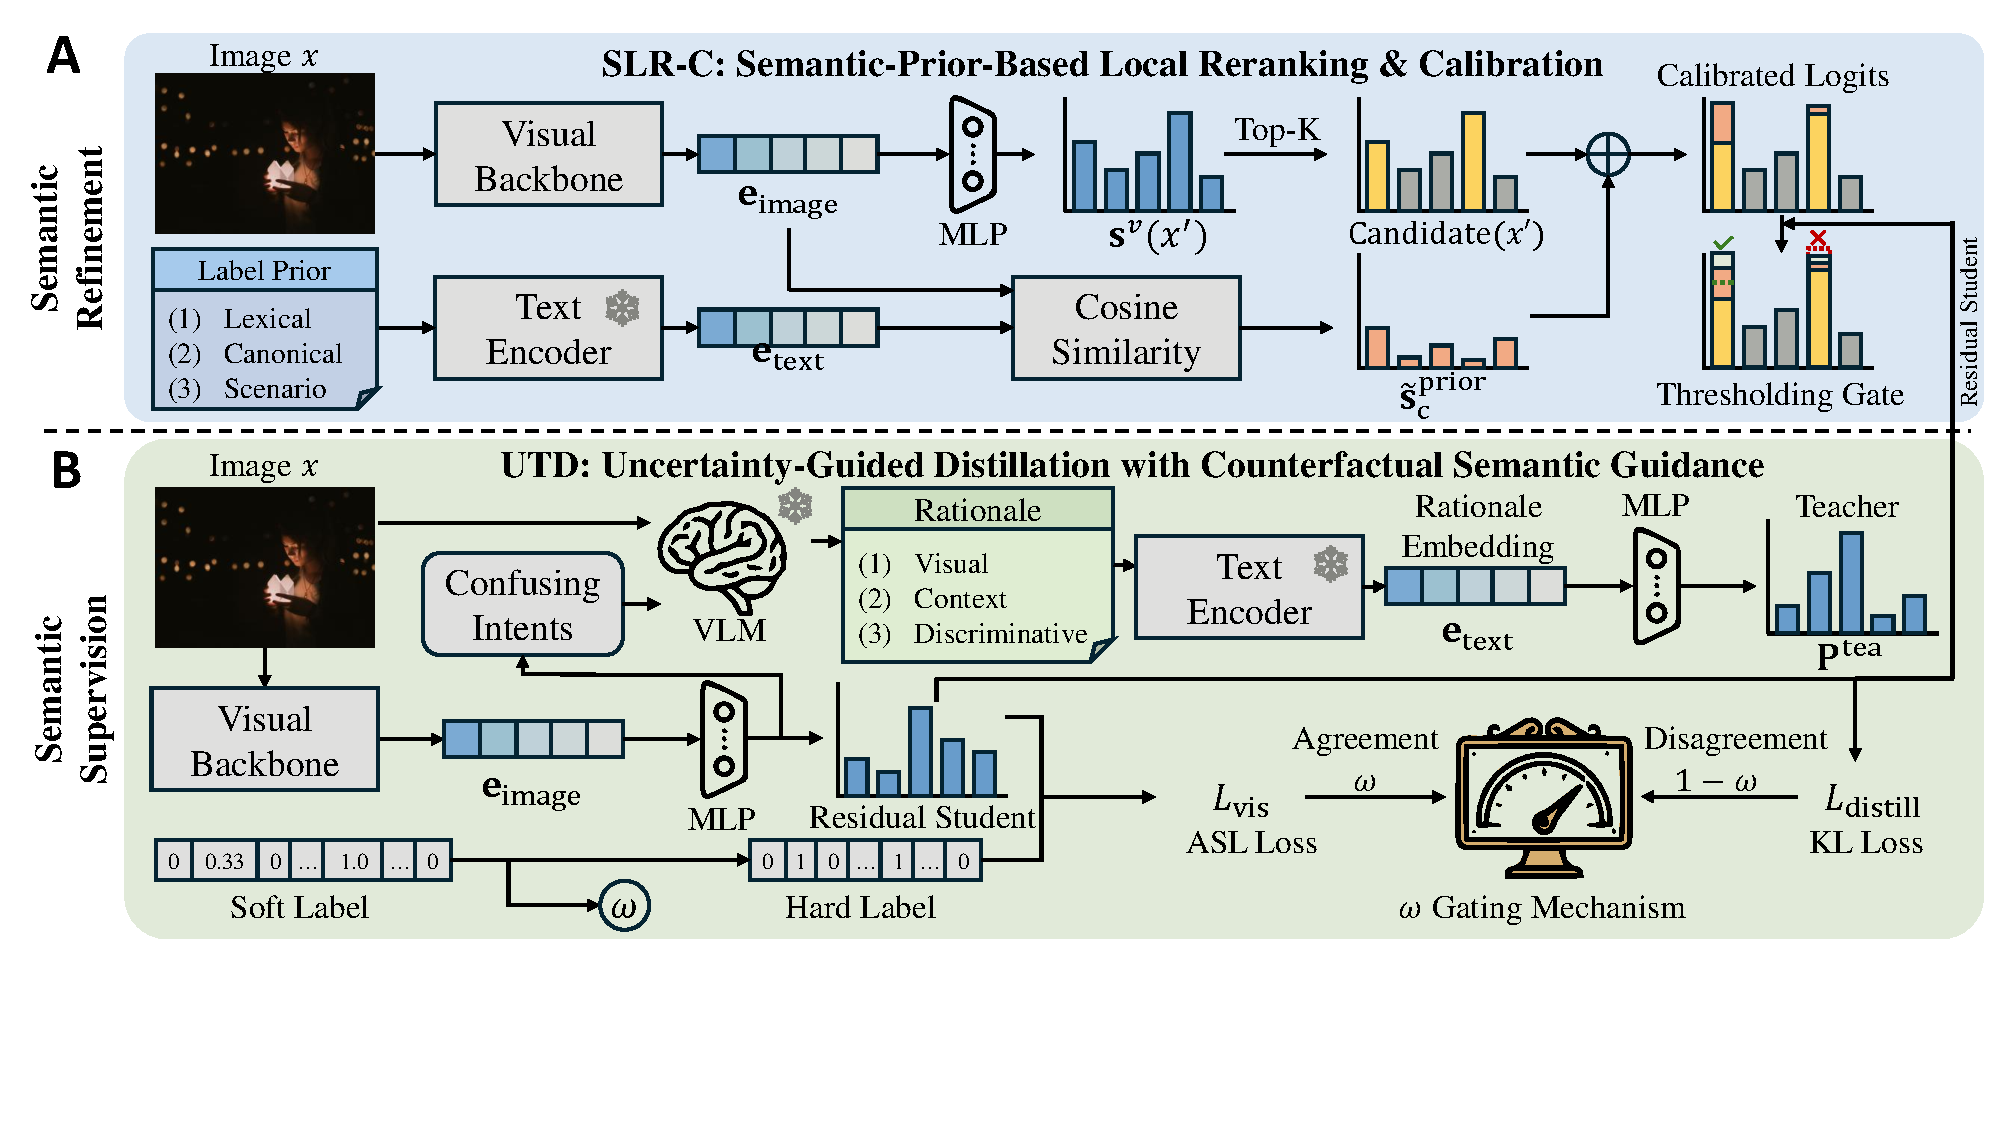
\includegraphics[width=\linewidth]{2_framework.pdf}
\caption{Overview of the FDIL framework. The framework functionally decouples ambiguity handling into \textbf{semantic refinement} (panel~A) and \textbf{semantic supervision} (panel~B). \revised{\textbf{(A, top) SLR-C module:}} heterogeneous lexical, canonical, and scenario priors define a semantic prior through Top-$K$ reranking, after which a lightweight residual student adapts the final prediction to image evidence before class-wise thresholding. \revised{\textbf{(B, bottom) UTD module:}} a VLM-derived text teacher provides rationale-based semantic supervision, and its contribution is adaptively gated by the annotator agreement score $\omega$ to stabilize learning under supervisory ambiguity.}
\label{fig:fdil_framework}
\end{figure}

\section{Method}
\label{sec:method}

\subsection{Overview}

To address the dual challenges of supervisory ambiguity and semantic ambiguity in visual intention recognition, we propose the \textbf{FDIL}, a functionally decoupled framework where fixed semantic priors provide structured candidate semantics, uncertainty-aware text teachers stabilize ambiguous supervision, and a residual student learns image-aware intent prediction on top of the semantic prior. Instead of forcing one unified mechanism to handle both supervisory ambiguity and semantic ambiguity, we assign them to two complementary functions.

FDIL consists of two key components, as shown in Figure~\ref{fig:fdil_framework}:
\begin{itemize}
    \item \textbf{Semantic Local Reranking and Calibration (SLR-C)}, which constructs a semantic prior from heterogeneous textual cues and supports image-aware refinement through a residual student;
    \item \textbf{Uncertainty-guided Text Distillation (UTD)}, which introduces adaptive semantic guidance to improve robustness under ambiguous supervision.
\end{itemize}

Given an input image, the model first produces visual intent scores using a strong visual backbone. SLR-C then provides structured candidate semantics by locally reranking intent candidates and forming a semantic prior. UTD supplies uncertainty-aware semantic supervision through a rationale-based text teacher and can be reused to regularize both the visual student and the residual refinement module built on top of the semantic prior.

\subsection{Problem Formulation}

Given an input image $x$, the goal is to predict a set of intent labels from a predefined label space $\mathcal{Y}=\{1,\dots,C\}$, where $C$ is the total number of intent categories. Due to the subjective nature of visual intention recognition, annotations are provided as soft label vectors $\mathbf{y}^{\text{soft}} \in \{0, 0.33, 0.66, 1\}^C$, reflecting annotator agreement.

Existing approaches typically follow either hard binarization or soft regression paradigms, both of which have limitations under ambiguous supervision. To address this, we adopt a \textbf{decoupled utilization} of annotation signals.

Specifically, we derive binarized labels $\mathbf{y}^{\text{hard}}$ for classification supervision, while extracting an image-level agreement score $\omega \in (0,1]$ from $\mathbf{y}^{\text{soft}}$. Here, $\omega$ reflects annotator consensus, where higher values indicate more reliable supervision. The binarized labels are computed as:
\begin{equation}
y^{\text{hard}}_{c} =
\begin{cases}
1, & \text{if } y^{\text{soft}}_{c} > 0 \\
0, & \text{otherwise}
\end{cases}
\end{equation}

In practice, an image may contain multiple positive intents with different agreement levels. We therefore adopt a conservative pooling rule and define the sample-level agreement as the minimum soft agreement among all positive labels:
\begin{equation}
\omega = \min_{c:\, y^{\text{hard}}_{c}=1} y^{\text{soft}}_{c}.
\end{equation}
This choice lets the hardest positive label determine how much the sample should trust direct supervision.

\subsection{Semantic Local Reranking and Calibration (SLR-C)}

Semantic ambiguity mainly manifests as local confusion among visually plausible but semantically adjacent intents. To address this, we first build a semantic refinement module that provides structured candidate semantics before turning to ambiguity-aware supervision.

\subsubsection{Semantic Prior Construction}

Intent semantics are inherently multi-granular and abstract, making a single textual representation insufficient. We therefore construct a heterogeneous semantic prior for each intent by combining three complementary textual sources: lexical intent phrases, canonical intent descriptions, and descriptive visual scenarios. The lexical source provides concise intent name cues, the canonical source provides semantic definitions, and the scenario source grounds abstract intents into plausible visual situations.


\paragraph{Example}
For the intent \textit{SocialLifeFriendship}, the \revised{lexical} phrase is \textit{``Social Life and Friendship''}, and the canonical description is:
\textit{``Being part of a social group. Having people to do things with. Having close friends, others to rely on. Making friends, drawing others near.''}
This intent can be further expanded into multiple scenario archetypes with distinct visual realizations:
\begin{quote}
\small
\textbf{Scenario 1}
\textit{``A photo of a group of friends hiking up a steep mountain trail together, wearing backpacks, laughing and giving high-fives under a bright sunny sky.''}

\textbf{Scenario 2}
\textit{``An image showing two close friends sitting on a comfortable living room couch, drinking coffee, leaning in closely to share a deep, supportive conversation.''}

\textbf{Scenario 3:}
\textit{``A photo of a large group of diverse people gathered around a busy dinner table, laughing loudly and toasting glasses of wine in a warmly lit room.''}

\textbf{Scenario 4:}
\textit{``An image showing a group of cheerful volunteers working together in a lush community garden, planting flowers side-by-side with dirty hands and bright smiles.''}
\end{quote}

\revised{\paragraph{Scenario selection and coverage.} The scenarios are not hand-picked illustrations but the output of a fixed generation protocol applied uniformly to every intent class (the exact instruction template is given in~\ref{app:scenario_prompt}). For each intent we ask the vision-language model to enumerate visually distinct realizations along five complementary axes -- subjects/objects, actions/interactions, settings/context, emotion/atmosphere, and photographic style -- and we explicitly require at least three different settings per intent so that the scenarios span the typical intra-class appearance variation rather than a single canonical view. The criterion for inclusion is therefore representativeness of the visual modes by which an intent is commonly expressed in social-media imagery, not exhaustive coverage of all possible situations. Two properties make this robust to incomplete coverage. First, the scenario source is only one of three prior sources and is combined by per-source normalization and averaging, so a class whose true scene is poorly covered still receives lexical and canonical evidence. Second, the prior is used only to \emph{rerank} a Top-$K$ candidate set and is further corrected by the trainable residual student; it never acts as a standalone classifier. Consequently, for a test image whose situation falls outside the generated scenarios, the expected behavior is graceful degradation rather than failure: the scenario term contributes little discriminative signal, the prediction falls back toward the base visual logits and the other two prior sources, and the residual student can still recover the correct intent from image evidence. This matches the ablation in Table~\ref{tab:prior_ablation}, where removing the scenario source lowers but does not collapse performance, and the multi-source ensemble is the most balanced choice.}

Given an image $x$, we compute image-text similarities as:
\begin{equation}
s^{\text{prior}}_c = \text{sim}(f_{\text{img}}(x), \mathbf{e}_c).
\end{equation}
In practice, $\text{sim}(\cdot,\cdot)$ is defined as the cosine similarity between L2-normalized image and text embeddings, and scaled by the CLIP logit scale $\gamma$, i.e.
\begin{equation}
\text{sim}(f_{\text{img}}(x), \mathbf{e}_c) = \gamma \cdot \frac{f_{\text{img}}(x)^\top \mathbf{e}_c}{\|f_{\text{img}}(x)\|_2 \|\mathbf{e}_c\|_2}.
\end{equation}

For each source, we obtain a class-wise similarity score and normalize it independently. Specifically, for source $r \in \{\text{lex}, \text{can}, \text{scen}\}$, we perform per-sample normalization across all classes:
\begin{equation}
\tilde{s}^{r}_c = \frac{s^{r}_c - \mu^{r}(x)}{\sigma^{r}(x) + \epsilon},
\end{equation}
where $\mu^{r}(x)=\frac{1}{C}\sum_{c=1}^{C}s^{r}_c$ and $\sigma^{r}(x)$ is the corresponding standard deviation over the $C$ intent classes, and $\epsilon$ is a small constant for numerical stability. The final prior is then constructed by averaging the normalized scores from the three sources as:
\begin{equation}
\tilde{s}^{\text{prior}}_c = \frac{1}{3}\left(\tilde{s}^{\text{lex}}_c + \tilde{s}^{\text{can}}_c + \tilde{s}^{\text{scen}}_c\right).
\end{equation}

\subsubsection{Semantic Local Reranking}

In the refinement module, we start from base visual logits $\mathbf{s}^{b}$ produced by a frozen visual student. We first select a compact candidate set as:
\begin{equation}
\mathcal{C}_K(x) = \text{TopK}(\mathbf{s}^{b}, K).
\end{equation}
The base logits are then locally adjusted with the normalized prior:
\begin{equation}
\tilde{s}_c =
\begin{cases}
s^{b}_c + \alpha \cdot \tilde{s}^{\text{prior}}_c, & c \in \mathcal{C}_K(x), \\
s^{b}_c, & \text{otherwise}.
\end{cases}
\end{equation}
Here $\alpha$ controls the strength of semantic reranking. In our implementation, $\alpha$ is fixed to 0.3.

This localized reranking produces a semantic prior that narrows the candidate set and sharpens the local score geometry without introducing an additional trainable prior module.

\subsubsection{Residual Refinement on the Semantic Prior}

Fixed reranking alone is not sufficient, because the heterogeneous prior may still fall short of the image-specific evidence. We therefore train a lightweight residual student on top of the semantic prior:
\begin{equation}
s^{\text{full}}_c = \tilde{s}_c + h_{\text{res}}(f_{\text{img}}(x))_c,
\end{equation}
where $h_{\text{res}}(\cdot)$ is a residual MLP that predicts class-wise residual intent scores from the image feature. In practice, the SLR-C logits $\tilde{s}_c$ are first computed and frozen, and the residual module is then optimized separately.

In the final full model, this residual module is not trained in isolation: it can also be regularized by the uncertainty-aware text teacher introduced next. Thus, SLR-C provides the structured candidate semantics first, and UTD later supplies the ambiguity-aware supervision used to stabilize image-aware prediction on top of the semantic prior.

\subsubsection{Class-wise Calibration}

Motivated by Guo et al. \cite{guo_calibration_2017}, to account for class imbalance and varying score distributions, we adopt class-wise thresholds:
\begin{equation}
\hat{y}_c = \mathbb{I}[\sigma(s^{\text{full}}_c) > t_c],
\end{equation}
where $t_c$ is determined on the validation set. Concretely, each threshold is selected independently by maximizing the class-wise validation F1 score:
\begin{equation}
t_c^\ast = \arg\max_{t \in \mathcal{T}} \text{F1}_c^{\text{val}}(t),
\end{equation}
where $\mathcal{T}$ is a fixed threshold grid. This design lets each class adapt its decision boundary to its own score distribution and frequency level, instead of sharing a single global threshold.

\subsection{Uncertainty-guided Text Distillation (UTD)}

%\subsubsection{Motivation}

Supervisory ambiguity arises when multiple plausible intents coexist for a given image. Direct optimization against hard labels may lead to overconfident predictions and unstable decision boundaries. To alleviate this issue, we introduce semantic guidance from text space and adapt its influence based on the uncertainty of supervision.

\subsubsection{Text-derived Teacher}

For each training image, we construct structured textual descriptions that capture semantic cues relevant to intention understanding. These descriptions are generated offline by a vision-language model, guided by both the image content and intent semantics.

To enhance discriminative capability under semantic ambiguity, we further incorporate contrastive cues by identifying visually plausible but incorrect intents predicted by the current model. Specifically, we select high-confidence negative intents as confusion candidates and use them to guide the generation of discriminative textual descriptions. This encourages the resulting text to emphasize subtle distinctions among semantically adjacent intents.

The generated text aims to summarize three aspects:
(1) observable visual elements,
(2) contextual interpretation beyond direct perception, and
(3) discriminative cues for distinguishing confusing intents.

The resulting text $T(x)$ is encoded into a dense embedding space using a frozen text encoder:
\begin{equation}
\mathbf{e}_{\text{text}} = f_{\text{text}}(T(x)).
\end{equation}

A lightweight classifier then maps the embedding into a multi-label teacher distribution:
\begin{equation}
\mathbf{p}^{\text{tea}} = \sigma(g_{\text{tea}}(\mathbf{e}_{\text{text}}) / \tau),
\end{equation}
where $\sigma(\cdot)$ is the sigmoid function and $\tau$ is the temperature parameter.

This design introduces contrastive semantic signals that improve the teacher's ability to distinguish semantically similar intents, while remaining separate from the semantic prior itself. In the full FDIL pipeline, the same teacher can further regularize the residual refinement module built on top of SLR-C.

\subsubsection{Uncertainty-guided Distillation}

The visual backbone produces logits $\mathbf{s}^{v}$ for image $x$. We adopt the Asymmetric Loss \cite{ridnik_asymmetric_2021} for classification:
\begin{equation}
\mathcal{L}_{\text{vis}} = \frac{1}{C} \sum_{c=1}^{C} \ell_{\text{ASL}}(s^{v}_{c}, y^{\text{hard}}_{c}).
\end{equation}

To incorporate semantic guidance, we introduce an uncertainty-guided Bernoulli distillation loss:
\begin{equation}
\mathcal{L}_{\text{distill}} = \sum_{c=1}^{C}\text{KL}\big(\mathrm{Bern}(p_c^{\text{tea}})\,\|\, \mathrm{Bern}(\sigma(s_c^{v}/\tau))\big),
\end{equation}
which is applied independently to each label. We use Bernoulli-style distillation rather than softmax distillation because intent recognition is a multi-label problem: each intent is modeled as an independent Bernoulli variable rather than as a mutually exclusive class on a probability simplex. This formulation preserves per-class uncertainty and avoids imposing artificial competition among labels.

Rather than mixing the two objectives with a fixed global coefficient, we use a gate derived from the agreement score. For the current sample, the teacher branch weight is defined as $g = 1 - \omega$, so low-agreement samples receive stronger semantic guidance, while high-agreement samples remain dominated by direct visual supervision.

Using $g$, the final loss is defined as:
\begin{equation}
\mathcal{L}_{\text{total}} = (1-g)\mathcal{L}_{\text{vis}} + \lambda g \mathcal{L}_{\text{distill}}
= \omega \mathcal{L}_{\text{vis}} + \lambda (1-\omega)\mathcal{L}_{\text{distill}}.
\end{equation}

This gated formulation allows the model to rely more on visual supervision when annotations are reliable, and to leverage semantic guidance when supervision is uncertain. In other words, UTD stabilizes ambiguous supervision through an uncertainty-aware text teacher rather than by modifying the semantic prior itself.

\subsection{Functionally Decoupled Ambiguity Modeling}
\label{sec:decoupling_principle}

We interpret visual intention recognition as a functionally decoupled ambiguity problem. Semantic ambiguity primarily distorts local candidate semantics, while supervisory ambiguity primarily destabilizes semantic supervision. \revised{Beyond this intuition, we now give an information-theoretic / feature-selection account of \emph{why} the two ambiguities are most naturally addressed by two separately parameterized functions rather than a single undifferentiated mechanism. The argument is a modeling \emph{principle} with testable predictions; it is not a claim that decoupling is the unique optimum, a point we revisit at the end of this subsection and verify empirically in Section~\ref{sec:experiments}.}

\revised{\paragraph{Setup.} Let $X$ denote the image, $\phi=f_{\text{img}}(X)\in\mathbb{R}^d$ its (frozen) representation, and $Y\in\{0,1\}^C$ the latent multi-label intent. The annotation process produces a soft target $\mathbf{y}^{\text{soft}}$ summarized by the hard labels $\mathbf{y}^{\text{hard}}$ and the agreement score $\omega\in(0,1]$ of Section~\ref{sec:method}. A predictor $g$ is restricted to functions of $\phi$, and is trained against the observed targets. The quantity that ultimately controls test error is the excess risk of $g\!\circ\!\phi$ relative to the Bayes intent posterior $\eta_c(x)=\Pr(Y_c{=}1\mid X{=}x)$.}

\revised{\paragraph{Two ambiguities are two distinct terms of the risk.} For class $c$, the per-sample excess risk admits a decomposition into a \emph{label-side} term and a \emph{feature-side} term:
\begin{equation}
\label{eq:risk_decomp}
\underbrace{\mathbb{E}\!\left[\ell\big(g_c(\phi),\, \tilde{y}_c\big)\right]}_{\text{training risk}}
\;\approx\;
\underbrace{\mathbb{E}_X\!\big[\mathcal{H}(\eta_c(X))\big]}_{\text{(S) supervisory: label-side entropy}}
\;+\;
\underbrace{\mathbb{E}_X\!\big[\,\eta_c(X)\,\text{aliasing}_c(\phi)\,\big]}_{\text{(F) semantic: feature-side aliasing}}
\;+\;\text{est.},
\end{equation}
where $\tilde{y}_c$ is the noisy annotation, $\mathcal{H}(\cdot)$ is the binary entropy, and ``est.'' collects the finite-sample estimation error. The two leading terms are governed by different objects. Term~(S) depends only on the conditional law $\Pr(Y\mid X)$: it is large precisely where annotators disagree, i.e.\ where $\mathcal{H}(\eta_c(X))$ is high, and it is \emph{irreducible by any function of $\phi$}---fitting harder against $\tilde{y}_c$ only converts this entropy into target noise and inflates the estimation term. Term~(F) depends only on the representation $\phi$: $\text{aliasing}_c(\phi)$ measures how much the feature map collapses class $c$ onto a semantically adjacent class $c'$, which we quantify by the inter-class mutual-information overlap
\begin{equation}
\label{eq:aliasing}
\text{aliasing}_c(\phi)\;\propto\;\max_{c'\neq c}\; I\big(\mathbf{1}[Y_c{=}1];\,\phi\big)\;-\;I\big(\mathbf{1}[Y_c{=}1];\,\phi \,\big|\, \mathbf{1}[Y_{c'}{=}1]\big),
\end{equation}
i.e.\ the part of the class-$c$ evidence in $\phi$ that is \emph{not separable} from a neighbor once that neighbor is known. Term~(F) is invariant to label noise and is reduced only by changing the decision geometry on the feature side.}

\revised{\paragraph{Principle (orthogonal corrections).} Because (S) is a functional of $\Pr(Y\mid X)$ and (F) is a functional of $\phi$, the two can be reduced by interventions with non-interfering first-order effects. Concretely, consider (i)~a \emph{label-side} reweighting that replaces the hard target by a reliability-weighted mixture with a teacher distribution, with weight a function of $\omega$ alone, and (ii)~a \emph{feature-side} restructuring that reranks and adds a residual to the decision scores as a function of $(\phi,\text{class text})$ alone. Under the mild condition that the gate depends only on $\omega$ and the prior/residual depend only on $(\phi,\text{class text})$---both satisfied by construction in FDIL---the Jacobians of the two interventions act on disjoint factors of Eq.~\eqref{eq:risk_decomp} (target distribution vs.\ score geometry), so to first order they neither cancel nor require trading one ambiguity against the other. A single scalar-weighted mechanism that mixes both signals into one supervision target cannot separate these factors and must compromise between them; a decoupled realization can drive each term with a dedicated, individually measurable module. This is the sense in which the decoupling is a \emph{principle} rather than an engineering convenience: it follows from which term of the risk each ambiguity occupies.}

\revised{\paragraph{Mapping to FDIL.} The two FDIL modules instantiate exactly these two interventions. \textbf{SLR-C} attacks term~(F): Top-$K$ reranking with the heterogeneous semantic prior $\tilde{s}^{\text{prior}}$ contracts the candidate set to the locally confusable neighborhood and sharpens its score geometry, while the residual $h_{\text{res}}(\phi)$ injects image-specific, class-discriminative directions---a feature-selection step that lowers $\text{aliasing}_c(\phi)$ within the candidate set. It is a function of $(\phi,\text{class text})$ only and does not touch the supervision target. \textbf{UTD} attacks term~(S): the agreement gate $g=1-\omega$ down-weights the direct visual loss exactly where $\mathcal{H}(\eta_c(X))$ is high and substitutes a smoother rationale-teacher distribution $\mathbf{p}^{\text{tea}}$, trading high-variance noisy targets for a lower-entropy surrogate. It is a function of $\omega$ (and offline text) only and does not alter the feature-side decision geometry. The decoupling in Eq.~\eqref{eq:risk_decomp} is therefore mirrored one-to-one in the architecture.}

\revised{\paragraph{Testable predictions.} The principle makes falsifiable predictions that we evaluate in Section~\ref{sec:experiments}. \textbf{(P1)~Separable, additive increments.} If the two modules act on different terms, each should yield an independent gain on a \emph{threshold-free} metric; we observe UTD alone $+2.40$ mAP and SLR-C a further $+2.03$ mAP, additively (matched-backbone group of Table~\ref{tab:main_results}). \textbf{(P2)~Content-dependence of the supervisory term.} Term~(S) is reduced by a teacher that carries genuine per-sample information; a teacher with matched \emph{form} but destroyed \emph{content} should not help and may hurt. The shuffled-rationale control is indeed the single most damaging intervention ($-7.8$ Macro F1, worse than removing the teacher; Table~\ref{tab:negative_controls}), ruling out an ``any external text'' explanation. \textbf{(P3)~Non-uniqueness of the realization.} The principle says the two terms must be \emph{addressed}, not that they must be \emph{physically separated}; a unified control that still respects both signals should approach a decoupled one on accuracy, but a control that collapses the two signals into a single mixed target need not. The unified-vs-decoupled comparison is consistent with both halves (Table~\ref{tab:unified_decoupled}): the strongest \emph{single-signal} unified control comes within about $0.6$ average F1 of FDIL, so decoupling is not the unique route to a competitive accuracy, whereas naively fusing both signals into one joint target underperforms the decoupled model and sits at the level of the weaker single signal. Decoupling's advantage is therefore primarily interpretability, separate measurability, and independent deployability, with a modest but consistent accuracy benefit over a single mixed target rather than a dramatically higher accuracy ceiling.}

FDIL addresses these two aspects through two different but compatible functions: SLR-C first provides structured candidate semantics through a semantic prior and residual refinement, while UTD supplies agreement-guided semantic supervision that stabilizes both the visual student and, in the full model, the residual refinement module built on top of the prior. This formulation is faithful to the current implementation, where the refinement module is optimized separately rather than jointly end-to-end with the teacher module.

This functionally decoupled design enables effective handling of ambiguity without introducing heavy architectural complexity.
